
\chapter{Evaluation and Lessons Learned}
\label{chap-eval}
To evaluate
our CertiKOS framework
and a series of verified kernels,
we have analyzed the performance  the  \cCTOS{} concurrent kernel
with a thorough experimental benchmark evaluation.
Furthermore, an extended version of \cCTOS{}
was deployed in a practical system that is used in the context of a
large DARPA-funded research project. 
Section~\ref{sec:eval:perform} shows our experiments with benchmarks, which
confirm the observations made during deployment: the performance
overhead of \cCTOS{} is moderate. 
In Section~\ref{sec:eval:impl},
we presents the implementation and deployment of
our verified kernels.
All in all, we are convinced that it is
practical to use our verification framework to produce competitive
real-world kernels with acceptable effort.


\section{Performance Evaluation} 
\label{sec:eval:perform}
Although the performance is not the main
emphasis of this thesis, we have run a number of micro and macro
benchmarks to measure the speedup and overhead of {\cCTOS} and to
compare {\cCTOS} to existing systems such as KVM and seL4. All
experiments have been performed on an Intel Core i7-2600S (2.8GHz,
4~cores) with 8~MB L3 cache, 16~GB memory, and a 120~GB
Intel 520 SSD. Since the power control code has not been verified, we
disabled the turbo boost and power management features of the hardware
during experiments.


\paragraph{Concurrency overhead} The run-time overhead introduced by concurrency
in {\cCTOS} mainly comes from \emph{the latency of spinlocks} and
\emph{the contention of the shared data}.

The {\cCTOS} kernel provides two kinds of spinlocks: ticket lock and
MCS lock. They have the same interface and thus are
interchangeable. In order to measure their performance, we put an
empty critical section (payload) under the protection of a single
lock. The latency is measured by taking a sample of 10,000 consecutive
lock acquires and releases (transactions) on each round.

\begin{figure}\centering
	\hspace{-.2cm}
	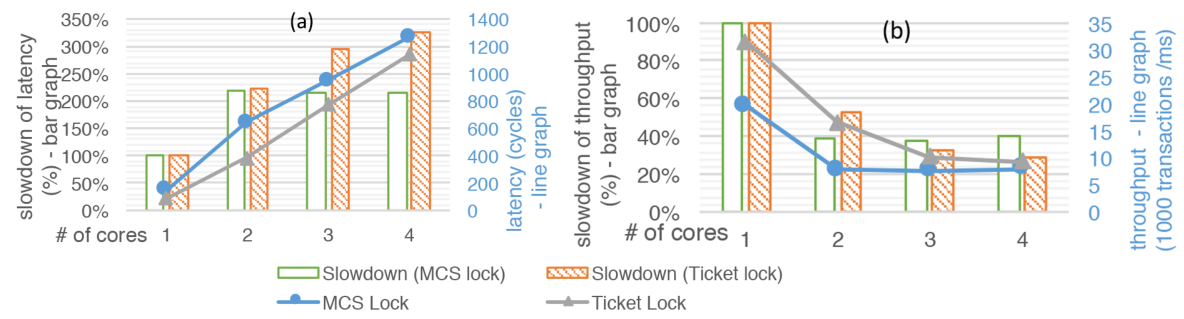
\includegraphics[width=10cm]{figs/locks.pdf}
	\hspace{-.2cm}
	\caption{The comparison between actual efficiency of ticket lock and MCS lock implementations in \cCTOS{}.}
	\label{fig:locks}
\vspace*{-10pt}        
\end{figure}

Figure~\ref{fig:locks} shows the results of our latency
measurement. In the single core case, ticket locks impose 34 cycles of
overhead, while MCS locks impose 74 cycles (line chart).
%%%%%%%%%%%%%%%%%%%%
\ignore{\hao{These numbers are larger
than normal spinning locks implementation. It is caused by the overhead of
additional primitive calls when we split the lock operation into multiple
layers.} \newman{Let's leave the numbers and comments for this for now.
Let's see if Hao can get the new performance data out before we submit
the report tonight. If not, we will revert the numbers back to the
old ones and add appropriate comments.}}
%%%%%%%%%%%%%%%%%%%%
As the number of cores grows, the latency increases rapidly. However,
note that all transactions are protected by the same lock. Thus, it is
expected that the slowdown should be proportional to the number of
cores. In order to show the actual efficiency of the lock
implementations, we normalize the latency against the baseline (single
core) multiplied by the number of cores ($\frac{n*t_1}{t_n}$). As can
be seen from the bar chart, efficiency remains about the same for MCS
lock, but decreases for ticket lock.

Now that we have compared MCS lock with ticket lock, we present the
remaining evaluations in this section using only the ticket lock
implementation of \cCTOS{}.

To reduce contention, all shared objects in {\cCTOS} are carefully
designed and pre-allocated with a fine-grained lock.
\ignore{
For example,
the {\cCTOS} process scheduler on each CPU does not need to access any
shared data if no relevant process is sleeping.
}
We design a benchmark
with server/client pairs to evaluate the speedup of the system as more
cores are introduced.  
We run a pair of server/client processes on each
core, and we measure the total throughput (i.e., the number of
transactions that servers make in each millisecond) across all
available cores.
%%%%%%%%%%%%%%%%
%In this benchmark, we run three pairs of server/client processes
%on all available cores, and we measure the total
%throughput (i.e., the number of transactions that servers make in each
%millisecond) across all the cores.
%%%%%%%%%%%%%%%%
A server's transaction consists of first performing an IPC receive
from a channel $i$, then executing a payload (certain number of
`\texttt{nop}' instructions), and finally sending a message to channel
$i + 1$. Correspondingly, a client sends an IPC message to channel
$i$, executes a constant payload of 500 cycles, and then receives its
server's message through channel $i + 1$.  When the client process has
to wait for a reply from the server, the control is switched to a
special system process which then immediately yields back to the server
process. 

\begin{figure}\centering
	\hspace{-.2cm}
	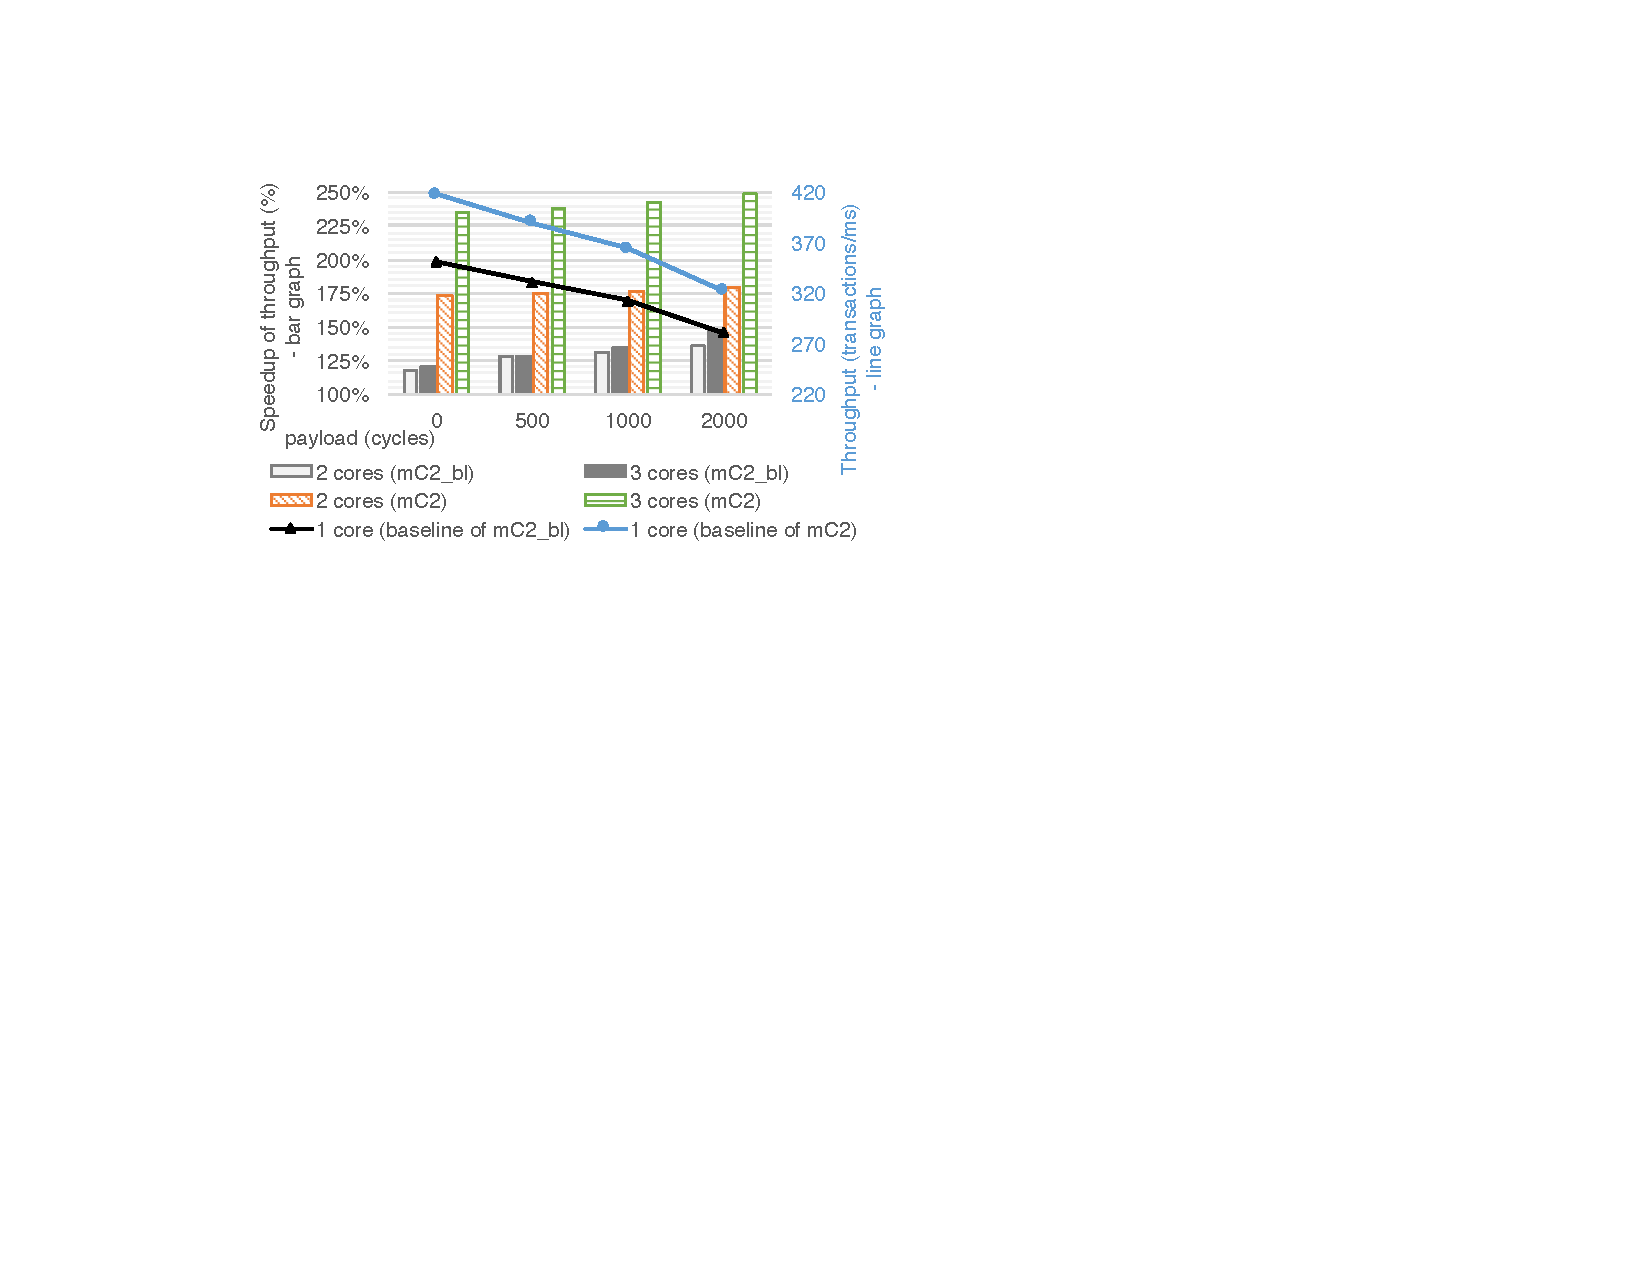
\includegraphics[width=10cm]{figs/speedup_big_lock.pdf}
	\hspace{-.2cm}
	\caption{Speedup of throughput of \cCTOS{} vs. {\cCTOS-bl} in a client/server benchmark under various server payloads (0-2,000).}
	\label{fig:speedup_big_lock}
\end{figure}


Figure~\ref{fig:speedup_big_lock} shows this server/client benchmark,
comparing {\cCTOS} against a big-kernel-lock version of {\cCTOS}
({\cCTOS-bl}). We insert a pair of lock acquire and release at the
top-most layer by hand, and replace all fine-grained locks with an
empty function. This does not introduce bias because the speedup is
normalized against its own baseline (single core throughput) for each
kernel version separately. From the figure, we can see that the
speedup rate for big-kernel-lock is about 1.54x $\sim$ 1.67x with 2
cores and 1.62x $\sim$ 2.05x with 3 cores. On the other hand, the
fine-grained locks of {\cCTOS} yield better speedup as the number of
cores increases (roughly 1.77x $\sim$ 1.85x and 2.63x $\sim$ 2.71x
with 2 and 3 cores, respectively). Note that the server/client pairs
are distributed into different CPUs, and there is no cross core
communication; therefore, one might expect perfect scaling as the
number of cores increases.  However, we do not quite achieve perfect
scaling because each core must execute some system processes which run
at constant rates and consume some CPU resources, and we did not align
our kernel data structures against cache-line size.

\ignore{
\begin{figure}\centering
	\hspace{-.2cm}
	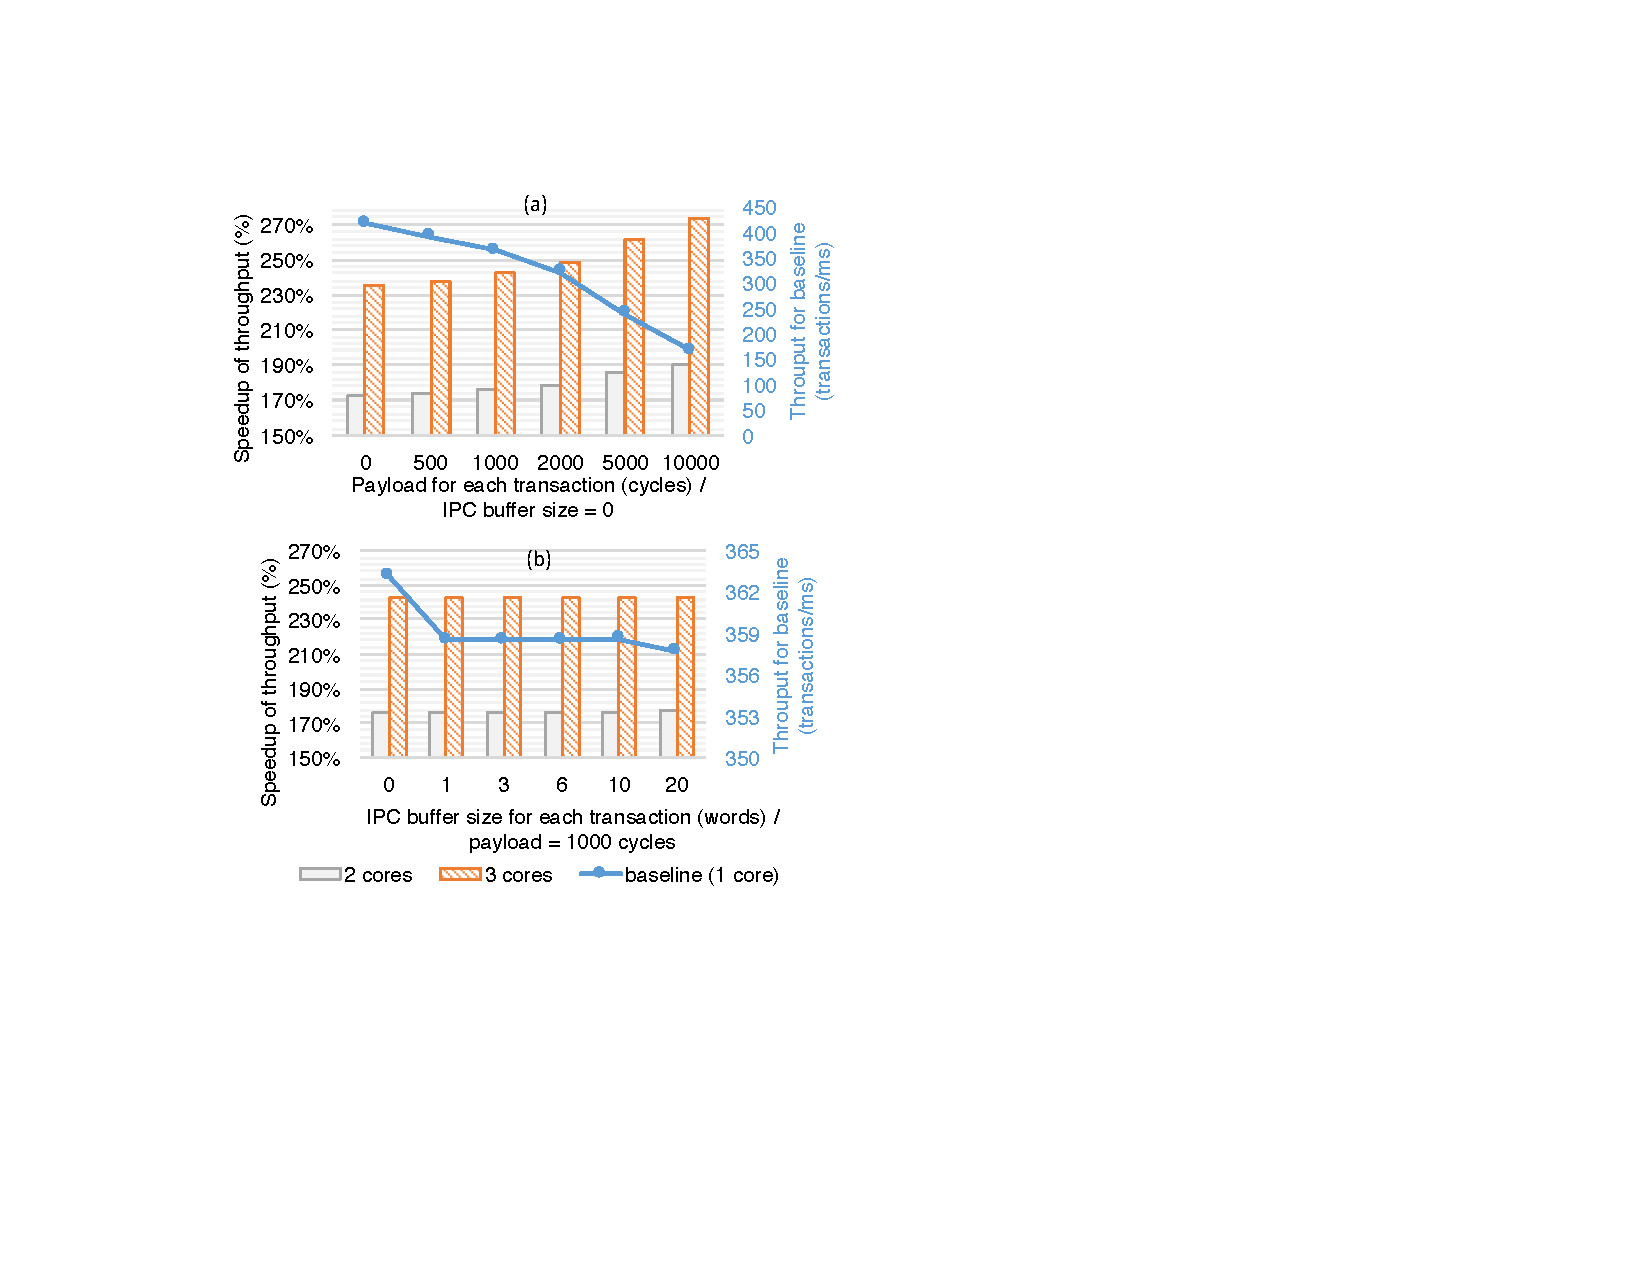
\includegraphics[width=6cm]{figs/speedup_pb.pdf}
	\hspace{-.2cm}
	\caption{Speedup of the throughput of \cCTOS{} in 2 and 3 cores against various server payloads (0 - 10,000) and IPC message sizes (0 - 20).}
	\label{fig:speedup_pb}
\end{figure}

Figure~\ref{fig:speedup_pb} shows the speedup of {\cCTOS} against various
server payloads and IPC message sizes. Figure~\ref{fig:speedup_pb} (a) shows that
the throughput decreases along with the increase of the server
workload (from I/O intensive task with payload being 0 to computation intensive task with
payload being 10,000) in the line chart. However, the speedup (bar chart) is increasing,
ranging from 1.7x to 1.9x for 2 cores, and 2.3x to 2.7x for 3 cores. The reason
is that the execution of the payload does not require the access to any shared
data, thus the contention becomes less intense. In
Figure~\ref{fig:speedup_pb} (b), the throughput decreases slightly when the
IPC message size increases, but the speedup is not affected.
}


\paragraph{IPC Performance} We measure the latency of IPC send/recv in {\cCTOS}
against various message sizes, and compare the result with seL4's IPC
implementation.

A comparison of the performance of seL4 and \cCTOS{} is not
straightforward since the verified \cCTOS{} kernel runs on a multicore
x86 platform, while the verified seL4 kernel runs on ARMv6 and ARMv7
hardware and only supports single-core. Thus, we use an unverified,
single-core version of seL4 for comparison. Moreover, the synchronized
IPC API in seL4 (\texttt{Call/ReplyWait}) has a different semantics
from \cCTOS{}'s send/recv: it uses a round-trip message passing
protocol (with a one-off reply channel created on the fly) while
trapping into the kernel twice, and it does not use any standard sleep
or wakeup procedures. To have a meaningful comparison with respect
to the efficiency of implementing system calls, we compare
$(send + recv) \times 2$
of \cCTOS{} with
${(Call + ReplyWait) + Null \times 2}$ of seL4,
where $Null$ is the latency of a null system call in seL4.

We measure seL4's performance using seL4's IPC benchmark
sel4bench-manifest~\cite{sel4bench} with processes in different
address spaces and with identical scheduler priorities, both in
\emph{slowpath} and \emph{fastpath} configurations. We consulted the
seL4 team~\cite{heiser16} and used 158 cycles as the cost of each null
system call ($Null$) in seL4. To measure \cCTOS{}'s performance, we
simply replace seL4's \emph{Call} and \emph{ReplyWait} system calls
with {\cCTOS}'s synchronous \emph{send} and \emph{receive} calls. We
found that, when the buffer size is zero, \cCTOS{} takes about 3800
cycles to perform a round trip IPC, while seL4's fastpath IPC takes
roughly 1200 cycles, and seL4's slowpath IPC takes 1800 cycles. When
the message size is larger than 2 words, the fastpath IPC of seL4
falls back to the slowpath; in the 10-words IPC case, \cCTOS{}'s round
trip IPC takes 3820 cycles, while seL4 takes 1830 cycles.
%%%%%%%%
\ignore{Considering \cCTOS{} requires two more system calls than
  seL4,\cCTOS{}'s IPC is slightly slower than seL4's.}
%%%%%%%%
Note that seL4 follows the microkernel design philosophy, and thus its
IPC performance is critical. IPC implementations in seL4 are highly
optimized and heavily tailored to specific hardware platforms.
%%%%%%%%
\ignore{The IPC performance of \cCTOS{} is still practical. Verification not
	only should not hinder application of similar performance optimizations, but
	instead provide a safety net for more aggressive optimizations, if it is
	required for application scenarios of the kernel we have in mind.}

\ignore{
	On {\cCTOS}, the performance of inter-core IPC is worse than that of
	intra-core IPC.  The reason is that, after the receiver thread is
	woken up, it is first pushed onto the \emph{pending queue} of the
	corresponding CPU, which gets pushed back to the scheduler's ready
	queue at the subsequent scheduling point. Furthermore, as shown in the
	figure, the performance of the send call is not affected by the buffer
	size. That is because the send system call simply saves the virtual
	address and size of the user buffer into the channel.  The actual
	copying of data is all done by the receive call.  Before copying the
	data, the receive call needs to switch the page map to an identity
	map, copy the data, and switch the page map back before it goes back
	to user. Note that switching page map causes TLB flushes, which
	imposes extra performance overhead to the receive call in addition to
	the overhead of copying the data.

\begin{figure}\centering
	\hspace{-.2cm}
	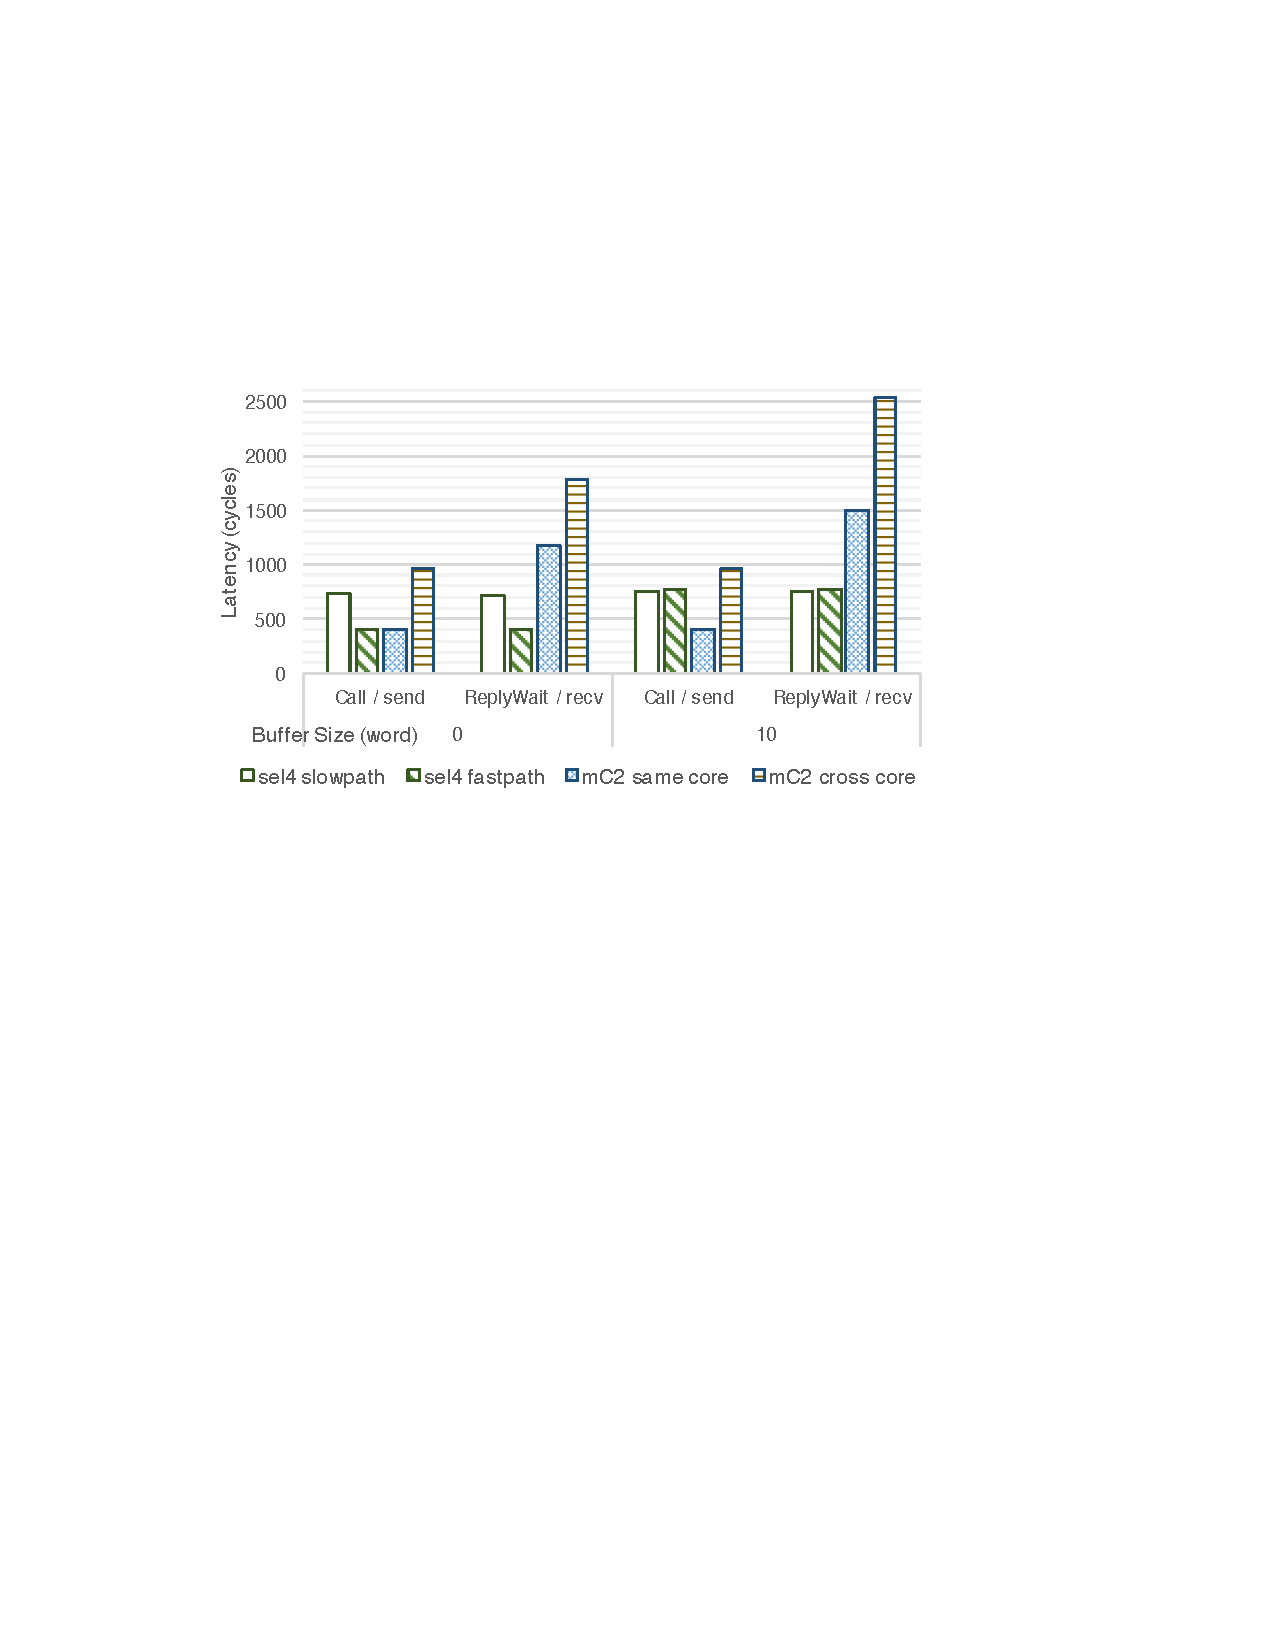
\includegraphics[width=8cm]{figs/ipc.pdf}
	\hspace{-.2cm}
	\caption{IPC performance between \cCTOS{} and  seL4 x86.}
	\label{fig:eval_ipc}
\end{figure}

}


\paragraph{Hypervisor Performance} 
\begin{figure}\centering
		\hspace{-.2cm}
		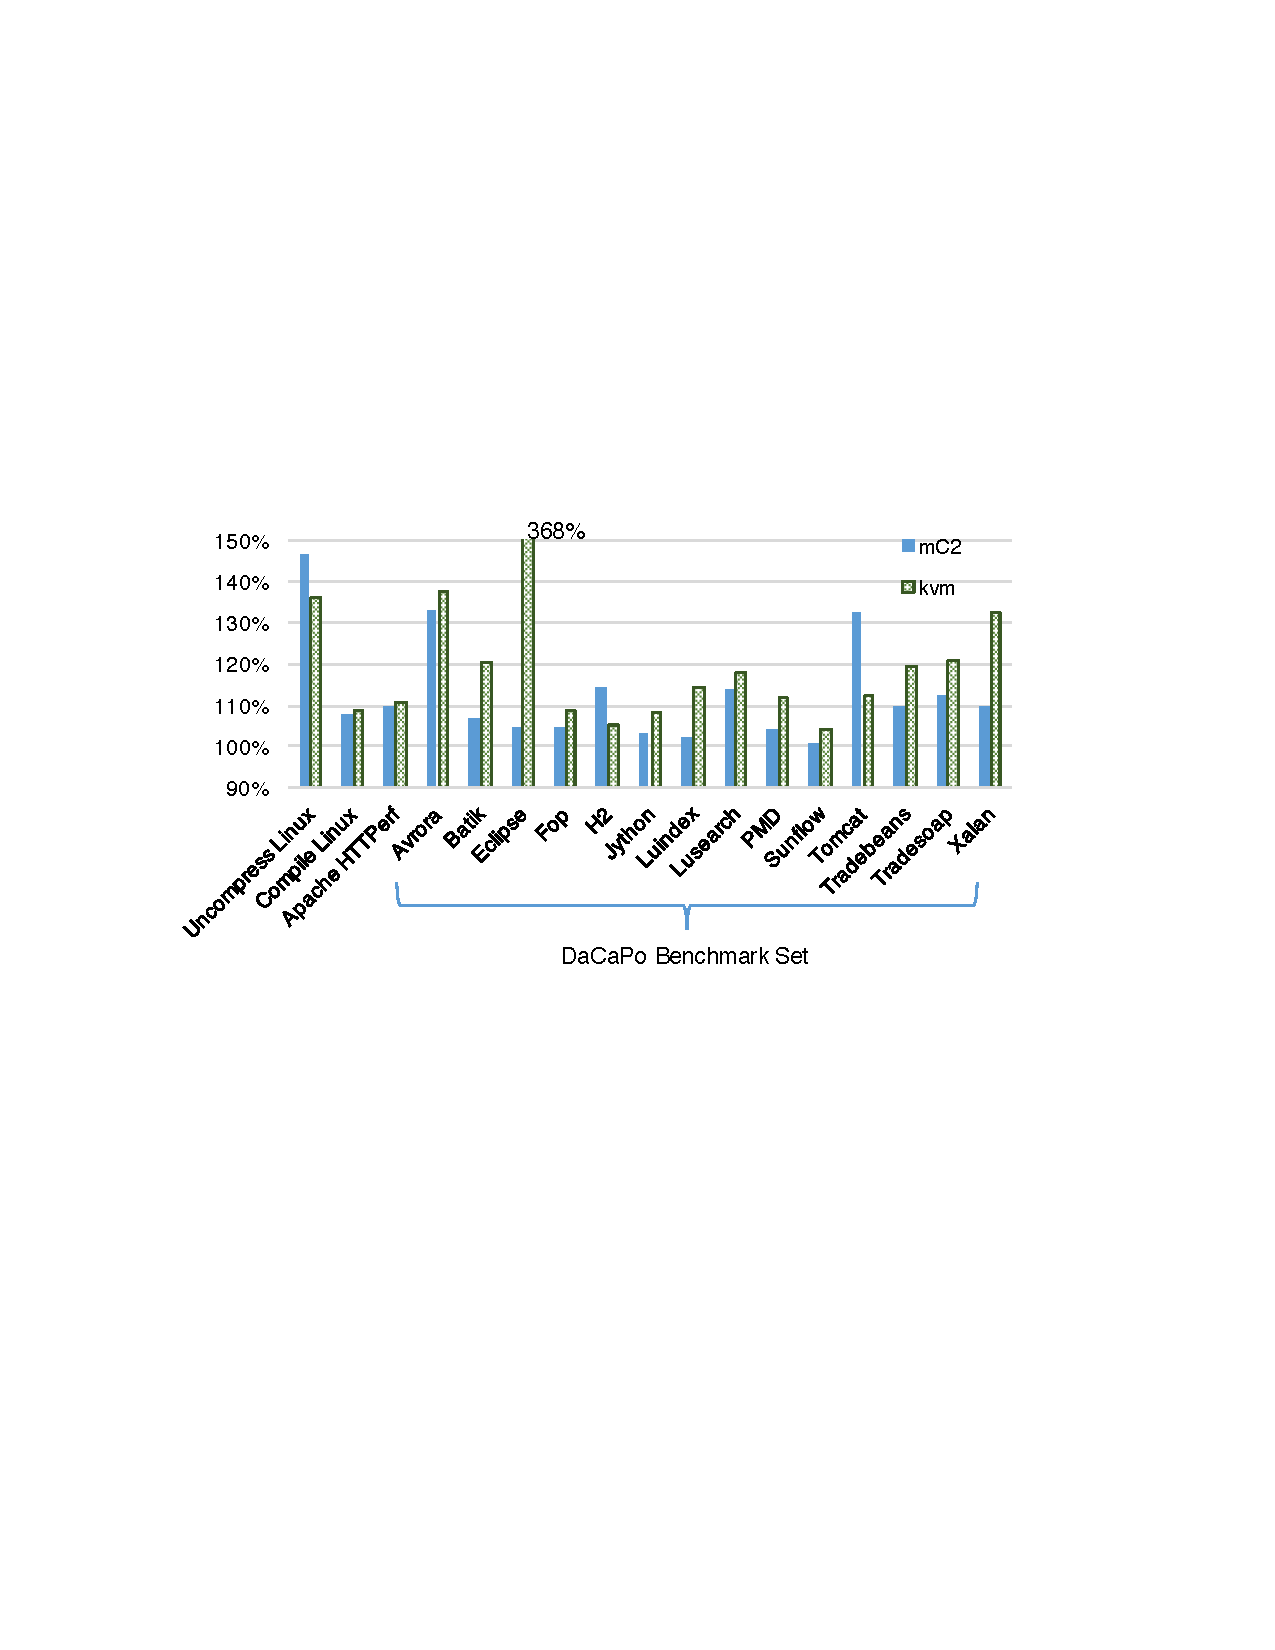
\includegraphics[width=13cm]{figs/hyp_macro.pdf}
		\hspace{-.2cm}
		\caption{Normalized performance for
                         macro benchmarks running over Linux on KVM
                         vs. Linux on \cCTOS; the baseline is
                         Linux on bare metal;
                         a smaller ratio is better.}
		\label{fig:eval_macro}
\end{figure}

To evaluate \cCTOS{} as a hypervisor, we measured the performance of some macro
benchmarks on Ubuntu 12.04.2 LTS running as a guest.  We ran the benchmarks on
Linux as guest in both KVM and \cCTOS{}, as well as on the bare metal. The guest
Ubuntu is installed on an internal SSD drive. KVM and \cCTOS{} are installed
on a USB stick. We use the standard 4KB pages in every setting~--- huge pages are not used.


 \ignore{Although there is an unverified branch of seL4 that supports
   VT-x, the verified version does not have virtualization support and
   cannot boot Linux. As a result, we do not compare hypervisor
   performance but instead focus on a comparison of the IPC
   performance of {\cCTOS} and an \emph{unverified} x86 version of
   seL4.}

Figure~\ref{fig:eval_macro} contains a compilation of standard macro
benchmarks: unpacking of the Linux 4.0-rc4 kernel, compilation of the
Linux 4.0-rc4 kernel, Apache HTTPerf~\cite{mosberger1998} (running on
loopback), and DaCaPo Benchmark 9.12~\cite{dacapo2006}.
%%%%%%%%%
\ignore{
To begin with a sanity check, McVoy's LMbench (version 3-alpha1) is used to
measure the micro-level metrics of operating system and hardware, which includes
the bandwidths and latency of several file system, local communication systems,
virtual memory, context switch and, basic arithmetic operations. The results
show that 34 out of 60 benchmarks of \cCTOS{} are very close to the bare
metal (within the range of 5\%), and the others are listed in the Table \hao{we need a talbe?}. These
results shows that there is no significant overhead of \cCTOS{}.
	}
%%%%%%%%%
% In Figure~\ref{fig:eval_macro}, w
%%%%%%%%%
We normalize the running times of the benchmarks using the bare metal
performance as a baseline (100\%). The overhead of \cCTOS{} is
moderate and comparable to KVM. In some cases, \cCTOS{} performs
better than KVM; we suspect this is because KVM has a Linux host and
thus has a larger cache footprint.  For benchmarks with a large number
of file operations, such as Uncompress Linux source and Tomcat,
\cCTOS{} performs worse. This is because \cCTOS{} expose the raw disk
interface to the guest via VirtIO~\cite{russell08} (instead of doing
the pass-through), and its disk driver does not provide good buffering
support.








\section{Implementation and Deployment}
\label{sec:eval:impl}
%\section{Implementation}
%\label{sec:imp}

\paragraph{Coq implementation}

After we finished the verification of different OS kernels presented
here, we have employed an exhaustive clean-up process to improve our
layered specification and verification framework.  Our initial Coq
implementation required verifying the contextual version of the
{\em implements} relation at each layer.  While such layer refinement
proofs followed some fixed patterns, the proof process heavily relied
on copying and pasting the existing templates and filling in the
missing proof holes.  The copy and paste approach also brought some
code and proof duplication.  In the new implementation, we instead
verify the per-primitive {\em implements} relation and then rely on the
soundness theorem of the layer calculus to turn this relation into the
contextual version. The contextual correctness property is derived
from the monotonicity of the client context in the carrier language.

We have also implemented more automation tactic libraries to further
ease the task of the verification. We are able to automate the majority of
tasks in the code verification and refinement proofs by extensively
applying these tactics. For the code verification, these tactics are
used for automatic definition unfolding, rewriting of terms, proving
that primitive calls never fault, verification condition generation,
and other first-order theorem proving to discharge the verification
conditions.  For the refinement relation, we developed a decision
procedure that automatically applies the layer calculus rules to split
the layer refinement into per-function forward simulations.  As for
the per-function forward simulation, getter-setter functions and
pass-through primitives are proved completely by tactic automations.
In the future, we are also interested in implementing horizontal
composition with framing to substitute the pass-through primitives.
We also built some extra libraries to prove x86 addressing modes and
the specification properties required by the layer calculus and
CompCertX.  Furthermore, we have extended the arithmetic
tactic \texttt{omega} with integer division and modulus.  Coq's
Ltac language is untyped, thus fixing a formal layer calculus helped a
lot in stabilizing these tactic libraries.

In our first approach, we tried to bundle the abstract data together
with the invariants on them using dependent types. This made the
automation of proofs more difficult as every time a new instance is
constructed, the framework requires us to explicitly construct a proof
that the new data satisfies the invariants. In our new approach, we
handle the invariants separately, and thus the invariants no longer
appear in the semantics of the primitives nor in the verification of
the programs. Then, we prove the layer interface invariant
preservation once and for all by showing that the initial abstract
data satisfies the invariants and all the semantics of the primitives
preserve the invariants. This proof makes sure that the layer
interface invariants are preserved during any execution, for all
programs (including the context) running on top of the layer
interface.


\paragraph{Proof effort}
With the help of the layer calculus and automation libraries
introduced in the new implementation, we successfully reduced the work
of adding one new layer from 4,000 lines of Coq code to 500 lines on
average.  The rough compilation time for a layer was reduced from a
few minutes to less than a minute.

The verification effort roughly falls into three categories: layer
design with specification and invariants, refinement proofs between
the layers, and verification of C and assembly code with respect to
the specifications. The time needed for each of the categories depends
largely on the layer.  For instance, at the boundary of physical and
virtual memory management ({$L_\code{MPTIntro}$}), almost all effort
is in the refinement proof, due to the proof for the refinement between
two completely different memory models. More effort went into the
refinement proof when we introduced the Intel \emph{virtual machine
memory model}, where we proved the refinement between the concrete
four level extended page table structure in memory and the abstract
mapping from the guest addresses to the host addresses.
In contrast, for the layer {\code{MATOp}},
which initializes physical memory allocation,
most of the time was spent on verifying
the non-trivial nested loops present in the C code,
while the refinement proofs were derived automatically. 

The proofs were facilitated by automation tools for C
code, layer design patterns, and tactics libraries developed in
recent years \cite{dscal15}. These tools have greatly
reduced the amount of work needed to verify extensions of the kernel.
\ignore{
\jeremie{I do not understand what the following sentence mean
(developing the module vs. ``plugging'' it),
I'm also not sure how it fits with the previous one,
I suggest we just drop it (or move it to Sec.5) and end the paragraph here.}
For example, developing the Intel virtualization module as a certified
kernel plug-in cost over 2 pm. However, plugging this module into
\mCTOSbase{} was done within a person week. \ignore{It took another 2 pm to
link all the proofs together and extract a runnable \mCTOShyper{}
assembly code using the Coq's extraction mechanism.} Modifying and
removing the existing modules does not take much effort either, as
demonstrated by the realization of \mCTOSringz{} and \mCTOSembed{},
which cost 0.5 pm each.
}



\paragraph*{Deployment}
An extended version of \mCTOShyper{} was deployed in context of a large
DARPA-funded research project. It runs on a military land vehicle
using the same hardware configuration we used in the experiments. On
top of the extended version run 6 Ubuntu Linux systems as guests. Each virtual
machine runs several RADL (The Robot Architecture Definition Language)
nodes that have fixed hardware capabilities such as access to GPS,
radar, \etc\\

\ignore{
This section describes our Coq implementation and provides some
actual evaluation of our various efforts. The main point of this
section to show that everything we have talked about so far are
actually real.

List of potential topics/discussions.
\begin{itemize}
\item Challenges met in the Coq implementation.
\item Particular interesting issues or challenges we met during the proof.
\item Any interesting topics we want to talk about in the proof.
\item How the new language constructs eased the task of verification/automation.
\item How we handle invariants. And how separating the invariants from the data helped the automation.
\item Bugs found?
\item Any implementation specific topics?
\item We we designed the layers.
\item Kernel specific challenges and/or interesting topics.
\item Modularity and scalability of our layered approach. How easy it was to extend the kernel with various new constructs?
\item Decide what to submit and acknowledge the work in progress and possible improvements.
\item \emph{anybody want to add more potential items here?}
\end{itemize}
}

\ignore{
\paragraph{Limitations and perspective}
We also try to enumerate all the important limitations of our current
effort. We want to address all possible questions typical readers of
our paper might have and explain why these issues can and will be
addressed in the future. 
}


\ignore{
\begin{figure}\small
\begin{center}
\begin{tabular}{|c|c|}
%\hline
%\multicolumn{2}{|l|}{Development of ClightX and CompCertX} & 10 pm \\
\hline
Physical memory module (3 layers) &  2 pm \\
\hline
Virtual memory module (7 layers) & 2.5 pm \\
\hline
Thread management (10 layers) & 3.5 pm \\
\hline
Process management (4 layers) & 1 pm \\
\hline
Trap handler module (3 layers) & 0.5 pm \\
\hline
\hline
Virtualization (9 layers) for \mCTOShyper{} & 1.5 pm \\
\hline
Changes for \mCTOSringz{}  & 0.5 pm \\
\hline
Changes for \mCTOSembed{}  & 0.5 pm\\
\hline
Linking and code extraction & 2 pm \\
\hline
\end{tabular}
\end{center}
\caption{Effort on verification}
\label{fig:effort}
\end{figure}
}

\ignore{
As shown in Fig.~\ref{fig:effort}, we completed the entire
verification effort of \mCTOS{} in less than 12 person months (pm).  At the
beginning, it took more than 2pm to design and verify the three layers
of physical memory management.  After the proof libraries (e.g. VCGen,
layer design pattern, tactics libraries \textit{etc}.) have been
developed, the average time of designing and verifying one layer was
dramatically reduced. On the verification side, one line of C code can
be proved within 30 lines of Coq code, while one line of assembly
requires only 20 lines of proof.
}



\paragraph{Execution Model and Completeness}
The majority of the {\cCTOS} and \cCTOS{} kernels are implemented and verified 
at the C level and then compiled by a modified version of the CompCert verified
compiler~\cite{dscal15}.  The entire kernel (both C and assembly)
source code, together with the source code for the verified compiler,
are extracted into an OCaml program through Coq's extraction
mechanism. When this OCaml program is executed, the extracted C source code 
is compiled into assembly; the resulting assembly code is then merged 
with the existing assembly kernel source code to produce a single piece 
of assembly code corresponding to our verified kernel.  Thus, our deliverable 
consists of a piece of assembly code for the entire verified kernel, a 
high-level deep specification of various kernel behaviors, and a 
machine-checkable proof object stating that the assembly code running on 
the actual hardware satisfies the high-level specification.

The verified assembly code is then linked with the rest of the kernel code
(the bootloader and remaining unverified drivers) to produce the
actual binary image of the OS. The resulting kernels are practical.

\begin{figure}[t]
\lstinputlisting [language = C, multicols=2] {source_code/fifoq3.c}
\caption{Pseudocode of the remove method for FIFOBBQ}
\label{fig:exp:fifo}
\end{figure}

\paragraph{Bugs found}
Formal verification is a great way to
locate hard-to-find concurrency-related bugs.
For example,  implementing starvation-free condition variables
is not trivial and even the popular, most up-to-date OS
textbook~\cite[Figure~5.14]{ospp11} has gotten it
wrong~\cite{anderson16}.

A \emph{condition variable} (CV) is a synchronization object that
enables a thread to wait for a change to be made to a
shared state (protected by a lock).  Standard Mesa-style
CVs~\cite{lampson80} do not guarantee starvation-freedom: a thread
waiting on a CV may not be signaled within a bounded number of
execution steps. 
Initially, we implemented a version of CV
using condition queues as shown by \citet[Figure~5.14]{ospp11}. However, during the verification,
we have found a bug in the FIFOBBQ implementation shown in that
textbook: in some cases, their system can get stuck by allowing all
the signaling and waiting threads to be asleep simultaneously, or the
system can arrive at a dead end where the threads on the remove queue
(rmvQ) can no longer be woken up.  We fixed this issue by postponing
the removal of the CV of a waiting thread from the queue, until the
waiting thread finishes its work (\cf Figure~\ref{fig:exp:fifo}); the
remover is now responsible for removing itself from the rmvQ (line~24)
and waking up the next element in the rmvQ (line~27). Here, \code{peekQ}
reads the head item of a queue; and \code{my\_cv} returns the CV
assigned to the current running thread. 

Other than the FIFOBBQ bug,
we have also found a subtle bug in  
our initial ticket-lock implementation:   
the spinning loop body (line 10 in Figure~\ref{fig:exp:ticket_lock})
was implemented as
``\lstinline$while($$\intp$\lstinline$L[i].now<t){}$". 
This still passed all our tests, but  
during the verification,
we found that it did not satisfy the atomic specification
since the ticket field might overflow. For example, 
if \lstinline$L[i].ticket$ is $(2^{32}-1)$, \code{acq\_lock} will
cause an overflow (line 9 in  Figure~\ref{fig:exp:ticket_lock}) and
the returned ticket
\lstinline$t$ equals $0$. In this case, 
\lstinline$L[i].now$ is not less than \lstinline$t$ 
and \code{acq\_lock} returns immediately, which violates 
the order implied by the ticket. We fixed this bug by 
changing the loop body to 
``\lstinline$while($$\intp$\lstinline$L[i].now!=t){}$";
we completed the proof by showing that the maximum 
number of concurrent threads is far below $2^{32}$.





\ignore{it
runs on stock x86 hardware and can successfully boot a guest version
of Linux.}

\ignore{\section{Proof effort}
We take the mCertiKOS kernel presented by Gu {\it et al}
\cite{dscal15}, and extend the kernel with various features such as
dynamic memory management, container support for controlling resource
consumption, Intel hardware virtualization support, shared memory IPC,
single-copy synchronous IPC, ticket and MCS lock implementation, new
schedulers, condition variables, FIFO blocking bounded queues, {\it
  etc}. Note that all of these new features are implemented in the
context of a concurrent machine, whereas the mCertiKOS presented by Gu
{\it et al} \cite{dscal15} only runs on a single-core machine. 

\ignore{ We
have also merged the work by Chen {\it et al} \cite{chen16} on the
interruptible kernel with device drivers using our multicore model.
}

Overall, we have contributed 3,500 additional lines of C and assembly
source code to the mCertiKOS code base. Regarding specification, there
are 943 lines of code used to specify the lowest layer axiomatizing
the hardware machine model, and 450 lines of code for the
specification of the abstract system call interfaces. These are in our
TCB and need to be trusted. We keep these specifications small to
limit the room for errors and ease the review process.  Outside the
TCB, there are 5249 lines of additional specifications for the various
kernel functions, and about 40K lines of code used to define auxiliary
definitions, lemmas, theorems, and invariants. Additionally, there are
50K lines of Coq proof scripts for proving the newly-added kernel
features. At least one third of these auxiliary definitions and proof
scripts are redundant and semi-automatically generated,\ignore{ (or
  copied and pasted),} which makes our proof a little verbose.  For
example, many invariant proofs get duplicated across the layers
whenever there is a minor change to the entire set of invariants.  We
are currently working on a new layer calculus to minimize redundant
definitions and proofs.

On the verification framework side, we developed a general linking
theorem for composing multiple threads running on the same CPU, as
well as a combining programs running on
different CPUs (10K lines).
Our team completed the verification of the new concurrent framework
and the additional features in about 2 person years. 
\ignore{It took 6 person
months to extend mCertiKOS with dynamic memory management, container
support, shared memory and synchronous IPC, and Intel
virtualization. The majority of the time (1.5 person years) was spent
on developing the framework to reason about the concurrent {\cCTOS}
kernel.} If we assume we work 250
days a year, we have written roughly 400 lines of code per
day\ignore{(50 lines per hour)}.  Thanks to the extensive layering,
the proofs for each small component are relatively easy; often it
takes less than two hours to write 400 lines of Coq code.  One of the
most challenging tasks is to come up with the correct specification
and invariants. In our experience, people make many mistakes when
initially writing down the specification; during the code verification
and refinement proof, we frequently find flaws in the specification or
notice that our invariants are too weak.  Furthermore, verification of
some components can be inherently complex, \eg, the kernel
initialization and locks.  It took us 3 days to certify the
ticket-lock acquire function (less than 10 lines of C code), and
multiple person weeks to prove that the ticket-lock is
starvation free.


Furthermore, note that we did not reach the current working solution
in one shot. We first spent about 3 person months developing an
unsuccessful version of the framework for composing multi-threaded
execution on a single CPU.  In that version, thread-local execution
was modeled using a \emph{time stamp} index into a global system
log. We eventually realized that the exact time stamps were too
cumbersome and revealed too much information about the underlying
implementation (\eg, the number of software yields within a function
body), so we spent another month developing a new system that uses
local logs (lists of events) instead.\ignore{ of time stamps, and the
  ability to shuffle and merge the events in the local logs to hide
  unnecessary nondeterminism or implementation details.}  Our initial
multicore machine model also did not work out very well when we
developed the multicore linking framework; we spent 3 person weeks to
improve the initial design through multiple iterations.  The main
challenge was finding the right invariants for the environment
context, such that we could successfully establish starvation-freedom.
}

\ignore{
\paragraph{Abstraction Layers}
\newman{I am gonna write some summary about the layered approach after I read
the overview section to see how much of the concepts are already covered.}
\ronghui{Maybe it is not helpful to include this part in the submission}
\begin{itemize}
\item Abstraction of data representation: doubly linked list --> logical list
\item Stronger invariants
\item Abstraction of primitive specification: hiding log implementation by linking and merging events
\item Refinement of machine models: from a realistic machine model to an ideal machine model that is suitable for our reasoning purpose, e.g., change in machine/memory/interrupt model
\end{itemize}
}

\ignore{
The verification effort roughly falls into three categories: layer
design with specification and invariants, refinement proofs between
the layers, and verification of C and assembly code with respect to
the specifications. The time needed for each of the categories depends
largely on the layer.  For instance, at the boundary of physical and
virtual memory management ({\code{MPTIntro}}), almost all effort
is in the refinement proof, due to the proof for the refinement between
two completely different memory models. More effort went into the
refinement proof when we introduced the Intel \emph{virtual machine
memory model}, where we proved the refinement between the concrete
four level extended page table structure in memory and the abstract
mapping from the guest addresses to the host addresses.
In contrast, for the layer {\code{MATOp}},
which initializes physical memory allocation,
most of the time was spent on verifying
the non-trivial nested loops present in the C code,
while the refinement proofs were derived automatically. 

The proofs were facilitated by automation tools for C
code, layer design patterns, and tactics libraries developed in
recent years \cite{dscal15}. These tools have greatly
reduced the amount of work needed to verify extensions of the kernel.
}


\ignore{\section{Extension and adaptation}
We augmented \cCTOSbase{} to support the hardware-assisted
virtualization technology Intel VT-x, and built a certified hypervisor
\cCTOShyper{}.  We have also built certified kernels with ring-0
process supports.  More details will be provided in the full paper.


First, we augmented \cCTOSbase{} to support the hardware-assisted
virtualization technology Intel VT-x, and built a
certified hypervisor \cCTOShyper{}. Second, we extended \cCTOSbase{}
into \cCTOSringz{} by adding support for
running certifiably-safe programs inside an ``in-kernel
process'' that runs in the privileged ring 0 mode.
We have also built \cCTOSembed{} kernel that is suitable for embedded systems,
by removing the virtual machine management and the virtual
memory management.
Removing plug-ins or layers are achieved simply by 
altering the contextual refinement proof 
at the boundary so that we can glue them back together.
}



%Bugs were found in the original design of $mCertiKOS$ during
%the C verification, which were not revealed during the original testing
%phase. They are mostly related to the overflow or the carelessness
%in implementation (e.g., writing \verb+x & y == 1+ instead of \verb+(x & y) == 1+).
% (Maybe talk about the necessity to have a separate initialization
%layer above intro layers before we introduce the layer implementing
%the actual operations???)
%Despite the frequent changes to the design, we found that the cost of change
%in our layered approach is quite small. (To compare with seL4, maybe mention
%adding new kernel modules, especially adding new kernel data structures to our
%layered design does not require significant changes to the original implementation
%of layers and the proofs.)


   % (a) Did the kernel actually run? If yes, what is the performance like?
   %     If the performance is not great, can we build a new version of
   %     our mCertiKOS kernel so that dramatically improves the performance?
   %     (note this optimized version of mCertiKOS does not have to be
   %      certified; we can explain what needs to be done in order to get
   %      this version certified and leave the actual verification to future
   %      work).

   % (b) Explain how it can manage to boot Linux; what are the key components
   %     and features in our current version of mCertiKOS that made this
   %     possible.

   % (c) Bootloader not verified, but see work by Cai et al;
   %     Stack-usage not verified, but see work by Carbonneaux et al;
   %     Interrupt handlers are ongoing work, see work by Feng et al and
   %     Guo et al. Device derivers not verified.



\ignore{
%\sectskip
\subsection{Extension and Adaptation}
\label{ssec:adapt}
%\asectskip

One primary advantage of our extensible architecture is that it makes
certified kernel extension and reasoning much easier and more principled. 
In this section, we first describe three alternative \cCTOSbase{} kernels
that we created through relatively minor changes to the base kernel. We
then present a specific example of global reasoning over the \cCTOSbase{} 
kernel~--- a simple notion of address space isolation that will serve as 
a starting point for a full-fledged security proof in the future.

We augmented \cCTOSbase{} to support the two hardware-assisted
virtualization technologies Intel VT-x and AMD SVM, and built a
certified hypervisor \cCTOShyper{}.

Fig. \ref{fig:base:vm:layers} shows the 7 layers of the virtual
machine management of \cCTOShyper{} on the Intel platform.
\code{VMInfo} is the layer object
that axiomatizes some of the hardware specific features needed
for the virtualization support. 
Since it is orthogonal to memory and process management,
the \code{VMInfo} object can be horizontally composed with the layers 
below \code{PProc} in \cCTOSbase{}.
On top of this extended \code{PProc} layer,
the virtual machine management extends the \emph{abstract memory model}
with the notions of Extended Page Table (EPT), the virtual machine
control structure (VMCS), and the virtual machine extension meta data (VMX),
which are abstracted into corresponding layer objects.
These objects are again orthogonal to the trap module above and can be
horizontally composed to export related system calls
with minimal cost.
 
\begin{figure}
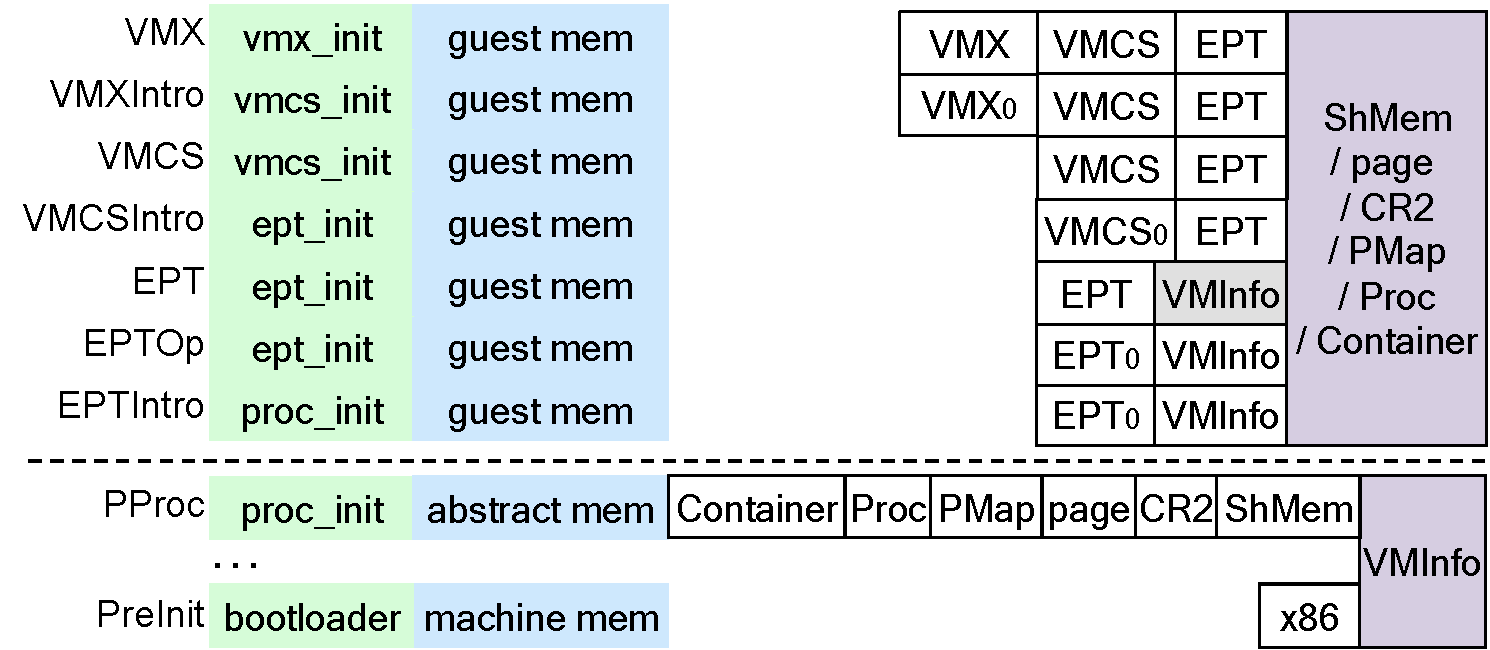
\includegraphics[scale=0.33]{figs/intel_layer}	
%\vspace*{-14pt}
\caption{Layers of virtual machine management}
\label{fig:base:vm:layers}
%\vspace*{-14pt}
\end{figure}

Thanks to the contextual refinement relation we have proved for
\cCTOSbase{}, one can certify user programs using our formal
specifications of system calls. This gives end-to-end proofs on
the behaviors of user programs when they run on \cCTOSbase{}.  
Furthermore, once certified, these processes can safely run in
the privileged ring 0 mode.  We extended \cCTOSbase{} into
\cCTOSringz{} by adding support for spawning ``in-kernel
processes'' that run in the privileged ring 0 mode. 
Ring 0 processes get much
better system call performance by directly calling kernel
functions and avoiding ring switch and interrupt processing. 

The \cCTOSembed{} kernel is intended for embedded settings. To develop
this kernel we started with \cCTOSringz{} and removed the virtual
machine management, the virtual memory management, and some of the
process management layers that are related to user contexts and user
process management.  Thus \cCTOSembed{} only supports ring 0 processes
which run directly inside the physical kernel address space instead of
the user-level paged virtual address space.

Removing plug-ins or layers does not take much effort.
We only need to alter the contextual refinement proof 
at the boundary so we can glue them back together.

\paragraph{Isolation in \cCTOSbase{}}
\label{security}
We have begun exploring the verification of a global security property
on top of \cCTOSbase{}. As a starting point, we proved a basic notion
of isolation between user-level processes running in different virtual
address spaces. This isolation property is composed of two theorems:
one regarding integrity (write protection), and another regarding
confidentiality (read protection, or noninterference).  The statements
of these two theorems are as follows: suppose the top layer abstract
machine takes one step, changing the machine state from $S$ to $S'$,
and let $p$ be the id of the currently-running process (which can be
found in $S$).
\begin{description}
  \item[Integrity:]
If the value at some non-kernel memory location $l$ differs between
$S$ and $S'$, then $l$ belongs to a page that is mapped in the 
virtual address space of $p$.
\item[Confidentiality:]
\label{confidential}
If the step taken
is not a primitive call to an IPC syscall (send, recv, etc.), then the values
of memory in any address space other than $p$'s cannot have an effect on the
result of the step. In other words, if we altered $S$ 
by changing data in a different process's address space, the step would still 
have the same effect on $p$'s address space.
\end{description}

In the future, we plan to provide a more detailed security policy by
describing what can happen to confidentiality when IPC is used.  This
description will be expressed in terms of propagation of security
labels on the IPC data. Note, however, that our framework allows for
security labels to be specified at a purely logical level~--- there is
no need for concrete representation and manipulation of labels at run
time.

Noninterference properties are generally not preserved across
refinement due to nondeterminism. It may therefore seem that the
aforementioned \emph{confidentiality} holds only at the topmost layer,
but not at lower layers. It turns out, however, that our notion of
deep specification is strong enough to preserve
noninterference. Essentially, to give a deep specification to a
nondeterministic semantics, we must first externalize the source of
nondeterminism (e.g., into an oracle). The noninterference property
then becomes parameterized over this source of nondeterminism, which
allows the parameterized property to be preserved across
refinement. This relationship between deep specification,
noninterference, and refinement will be explored comprehensively in
future work.
}

